%=== Results_and_Discussion ===
%=== (Actual work done and contribution, including literature survey) ===

\chapter{Experiments and Results}

\section{Experiments}
We experimented with a number of SED systems, using different variations of the spectrogram representation, data augmentation technique, model type,  post-prediction method and threshold type. All the experiments were done on the higher quality dataset, with audio clips of 16k Hz. We evaluated these SED systems on the test set of the project dataset mentioned in Section 3.1. The test set consists of 747 audio clip files, each around 10 seconds long.\\ 

We conducted the experiments in a sequential manner, that is, we first experimented with the audio features, with other variables constant. Once the best audio feature type is determined, we move on to experiment with the data augmentation techniques, followed by model types, then threshold types, and finally the post-prediction processing methods. Ideally, we would have experimented with all the different combinations of the variables to determine the best-performing system. However, we were unable to do so due to time and resource constraints.\\ 
% Hence, we performed the experiments sequentially instead.\\

In order to make the experiments more comprehensive, we also evaluated the best-performing SED system with the lower quality dataset, with 8k Hz audio clips, mentioned in Section 3.1.1. In this evaluation, our SED system is trained from scratch using the lower quality 8k Hz dataset, and then evaluated on the corresponding test set. This is done to determine how the SED system would perform with data we would more likely obtain in real-life scenarios.\\

Next, we evaluated the best-performing SED systems, based on the 16k Hz project dataset, on the DCASE 2017 Task 4 dataset in order to determine whether our proposed systems are comparable with state-of-the-art systems as well. In this evaluation, our SED system is trained from scratch again using the DCASE 2017 training set, which consists of 51,172 weakly-labelled audio clips, validated using the validation set, consisting of 488 clips and then evaluated on the test set, which contains 1,103 clips. Each audio clip is around 10 seconds long.\\

Finally, we evaluated our SED system on longer audio clips in order to observe the effects of our proposed pre-prediction and post-prediction processing method on them. However, as it is costly and very time consuming to annotate audio clips with strong labels, we only evaluated two 1-minute long audio clips, which is 6 times longer than the 10 second long audio clips in our project dataset. These two audio clips, which are independent of the audio clips in the development dataset, were downloaded from YouTube and manually-labelled ourselves.

\section{Evaluation Metric}
The evaluation metric used in this thesis follows the metric used in the DCASE 2017 Task 4 challenge \cite{DCASE2017}, which is segment-based evaluation with error rate and F1-score. The segment-based evaluation is done in a fixed time grid, in which segments of one second length are used to compare the groundtruth and system output. In each segment k, we count the number of each of the following values:
\begin{itemize}

\item{true positives (TP) - active events as indicated by both the ground truth and system output;}
\item{false positives (FP) - active events as indicated by the system output but inactive according to the ground truth;}
\item{false negatives (FN) - inactive events as indicated by the system output but active according to the ground truth;} 
\item{substitutions (S) - occur when the system output wrongly indicates an event as active; one substitution is equivalent to one FP and one FN, which means that the system did not detect the correct event (FN for the correct class) but detected something (FP for another class);}
\item{insertions (I) - number of FPs after subtracting the substitutions;}
\item{deletions (D) - number of FNs after subtracting the substitutions;}
\item{reference events (N) - number of sound events in the ground truth.}

\end{itemize}

\subsection{Error Rate}
The computation of the error rate ER follows the formula described in \cite{Poliner2007}. It is calculated over all the test data using the total number of insertions I, deletions D and substitutions S, and is formulated as follows:
\begin{equation}
ER = \sum{S(k)} + \sum{D(k)} + \sum{I(k)}\sum{N(k)}.    
\end{equation}

\subsection{F1-Score}
The F1-score F can be described as the harmonic mean of the precision P and recall R scores. It is calculated over all the test data based on the total number of false positives FPs, false negatives FNs, and true positives TPs, and is formulated as follows:
\begin{equation}
F = \frac{2(P \times R)}{P + R},
\end{equation}

where \(P = \frac{\sum{TP(k)}}{\sum{TP(k)} + \sum{FP(k)}}\) and \(R = \frac{\sum{TP(k)}}{\sum{TP(k)} + \sum{FN(k)}}\).

\section{Results}

This section summarises the results of the experiments conducted for this project.

\subsection{Results for Different Audio Feature Types}
The data augmentation technique, model type, threshold type, and pre-prediction and post-prediction processing method are constant and set to SpecAugment with mixup, 9-layer CNN with GRU and attention aggregation, non-optimised thresholds, and none, respectively. The results of the experiment with the varied audio feature types are summarised in Table \ref{tab:spec-res}.

\begin{table}[!htp]
\centering
\begin{tabular}{|c|c|c|c|c|}
\hline
\textbf{Spectrogram Representation}                         & \textbf{Error Rate}                                   & \textbf{F1-Score}                                     & \textbf{Precision}                                    & \textbf{Recall}                                       \\ \hline
\begin{tabular}[c]{@{}c@{}}Log-mel\\ Gammatone\end{tabular} & \begin{tabular}[c]{@{}c@{}}\textbf{0.555}\\ 0.569\end{tabular} & \begin{tabular}[c]{@{}c@{}}\textbf{0.624}\\ 0.605\end{tabular} & \begin{tabular}[c]{@{}c@{}}0.718\\ \textbf{0.732}\end{tabular} & \begin{tabular}[c]{@{}c@{}}\textbf{0.552}\\ 0.516\end{tabular} \\ \hline
\end{tabular}
\caption{\label{tab:spec-res}Comparison of spectrogram representations}
\end{table}

% \begin{table}[!htp]
%     \scriptsize
%     \centering
%     \begin{tabularx}{\textwidth}{llrlRRRRRR}
% \toprule
% &Spectrogram Representation& 
%         Segment-based Error Rate &
%                 Segment-based F1-Score &
%                         Precision&    Recall&    SAR&    STOI &  ESTOI & WER\\ \midrule
% \multirow{9}{*}{\makecell[cl]{\rotatebox{90}{Raw}}}
% &\multirow{1}{*}{\makecell[cl]{Log-mel}} &
% \multirow{1}{*}{0.555}&
% 0.624 &0.718    &0.552\\
% \cline{2-10}
% &\multirow{1}{*}{Gammatone} &
% \multirow{1}{*}{0.569}&
% 0.605 &0.732    &0.516\\
% \cline{2-10}

% \bottomrule
%     \end{tabularx}
%     \caption[Performance summary for two-source separation]{Performance summary for two-source separation\\}
%     \label{tab:summary2}
% \end{table}

\subsection{Results for Different Data Augmentation Techniques}
From the preceding experiment, we have determined that using the log-mel spectrogram representation produced a better performing system. As such, it is used as the audio feature in the following experiments. The model type, post-prediction processing method, and threshold type are the same as those in the preceding experiment. The results of the experiment with the varied data augmentation techniques are summarised in Table \ref{tab:data-aug-res}.\\

\begin{table}[!htp]
\centering
\resizebox{\textwidth}{!}{\begin{tabular}{|c|c|c|c|c|}
\hline
\textbf{Data Augmentation Technique}                                                                                                                                                          & \textbf{Error Rate}                                                                                   & \textbf{F1-Score}                                                                                     & \textbf{Precision}                                                                                    & \textbf{Recall}                                                                                       \\ \hline
\begin{tabular}[c]{@{}c@{}}None\\ SpecAugment\\ Mixup\\ Time-shift\\ SpecAugment \& Mixup\\ SpecAugment \& Time-shift\\ Mixup \& Time-shift\\ SpecAugment \& Mixup \& Time-shift\end{tabular} & \begin{tabular}[c]{@{}c@{}}0.599\\ 0.592\\ 0.567\\ 0.614\\ \textbf{0.555}\\ 0.599\\ 0.606\\ 0.583\end{tabular} & \begin{tabular}[c]{@{}c@{}}0.589\\ 0.600\\ 0.611\\ 0.563\\ \textbf{0.624}\\ 0.596\\ 0.569\\ 0.598\end{tabular} & \begin{tabular}[c]{@{}c@{}}0.674\\ 0.660\\ \textbf{0.740}\\ 0.698\\ 0.718\\ 0.670\\ 0.730\\ 0.727\end{tabular} & \begin{tabular}[c]{@{}c@{}}0.523\\ \textbf{0.551}\\ 0.521\\ 0.472\\ 0.552\\ 0.536\\ 0.466\\ 0.507\end{tabular} \\ \hline
\end{tabular}}
\caption{\label{tab:data-aug-res}Comparison of data augmentation techniques}
\end{table}

\subsection{Results for Different Model Types}
From the preceding experiments, we have determined that the log-mel spectrogram representation and SpecAugment with mixup produced a better performing system. As such, they are used as the audio feature and data augmentation technique, respectively, in the following experiments. The threshold type and post-prediction processing method are the same as those in the preceeding experiment. The results of the experiment with the varied model types are summarised in Table \ref{tab:model-res}.

\begin{table}[!htp]
\centering
\resizebox{\textwidth}{!}{\begin{tabular}{|c|c|c|c|c|c|}
\hline
\textbf{Model}                                                                                                                                                                                                                                                                                                         & \textbf{Error Rate}                                                                                                           & \textbf{F1-Score}                                                                                                             & \textbf{Precision}                                                                                                            & \textbf{Recall}                                                                                                               & \textbf{\begin{tabular}[c]{@{}c@{}}Model Size\\ (\# parameters)\end{tabular}}                                                                                                \\ \hline
\begin{tabular}[c]{@{}c@{}}CNN-9-GRU-Attention\\ CNN-9-GRU-Average\\ CNN-14-GRU-Attention\\ CNN-9-Transformer-Attention\\ CNN-9-Transformer-Average\\ CNN-14-Transformer-Attention\\ CNN-9-Conformer-Attention\\ CNN-9-Conformer-Average\\ CNN-14-Conformer-Attention\\ VGGish-Attention\\ VGGish-Average\end{tabular} & \begin{tabular}[c]{@{}c@{}}0.555\\ 0.604\\ 0.590\\ \textbf{0.552}\\ 0.633\\ 0.559\\ 0.560\\ 0.638\\ 0.584\\ 0.681\\ 0.676\end{tabular} & \begin{tabular}[c]{@{}c@{}}0.624\\ 0.591\\ 0.585\\ \textbf{0.628}\\ 0.544\\ 0.617\\ 0.620\\ 0.555\\ 0.596\\ 0.506\\ 0.520\end{tabular} & \begin{tabular}[c]{@{}c@{}}0.718\\ 0.664\\ 0.714\\ 0.712\\ 0.696\\ \textbf{0.732}\\ 0.666\\ 0.627\\ 0.682\\ 0.672\\ 0.618\end{tabular} & \begin{tabular}[c]{@{}c@{}}0.552\\ 0.532\\ 0.495\\ 0.562\\ 0.447\\ 0.533\\ \textbf{0.580}\\ 0.497\\ 0.530\\ 0.406\\ 0.448\end{tabular} & \begin{tabular}[c]{@{}c@{}}5,894,692\\ 5,881,817\\ 94,466,596\\ 5,763,620\\ 5,750,745\\ 79,781,924\\ 6,280,493\\ 6,276,818\\ 77,295,917\\ 5,708,260\\ 5,695,385\end{tabular} \\ \hline
\end{tabular}}
\caption{\label{tab:model-res}Comparison of model types}
\end{table}

\subsection{Results for Applying Optimised Thresholds}
From the preceding experiment, we determined that the 9-layer CNN with Transformer, the 9-layer CNN with Conformer, and 9-layer CNN with GRU models, all with attention aggregation applied, produced the better performing models. We tested these three models in the following experiments, while keeping the audio feature and data augmentation technique used the same as those in the preceding experiment. No pre-prediction or post-prediction processing methods are applied. The results of the experiment of applying the optimised thresholds are summarised in Table \ref{tab:thres-res}.

\begin{table}[!htp]
\centering
\begin{tabular}{|c|c|c|c|c|c|}
\hline
\textbf{Model}                                                            & \textbf{Threshold Type}                                           & \textbf{Error Rate}                                   & \textbf{F1-Score}                                     & \textbf{Precision}                                    & \textbf{Recall}                                       \\ \hline
\begin{tabular}[c]{@{}c@{}}CNN-9\\ -GRU\\ -Attention\end{tabular}         & \begin{tabular}[c]{@{}c@{}}Non-optimised\\ Optimised\end{tabular} & \begin{tabular}[c]{@{}c@{}}0.555\\ 0.601\end{tabular} & \begin{tabular}[c]{@{}c@{}}0.624\\ 0.635\end{tabular} & \begin{tabular}[c]{@{}c@{}}\textbf{0.718}\\ 0.619\end{tabular} & \begin{tabular}[c]{@{}c@{}}0.552\\ \textbf{0.651}\end{tabular} \\ \hline
\begin{tabular}[c]{@{}c@{}}CNN-9\\ -Transformer\\ -Attention\end{tabular} & \begin{tabular}[c]{@{}c@{}}Non-optimised\\ Optimised\end{tabular} & \begin{tabular}[c]{@{}c@{}}\textbf{0.552}\\ 0.561\end{tabular} & \begin{tabular}[c]{@{}c@{}}0.628\\ \textbf{0.648}\end{tabular} & \begin{tabular}[c]{@{}c@{}}0.712\\ 0.650\end{tabular} & \begin{tabular}[c]{@{}c@{}}0.562\\ 0.646\end{tabular} \\ \hline
\begin{tabular}[c]{@{}c@{}}CNN-9\\ -Conformer\\ -Attention\end{tabular}   & \begin{tabular}[c]{@{}c@{}}Non-optimised\\ Optimised\end{tabular} & \begin{tabular}[c]{@{}c@{}}0.560\\ 0.591\end{tabular} & \begin{tabular}[c]{@{}c@{}}0.620\\ 0.629\end{tabular} & \begin{tabular}[c]{@{}c@{}}0.675\\ 0.617\end{tabular} & \begin{tabular}[c]{@{}c@{}}0.599\\ 0.642\end{tabular} \\ \hline
\end{tabular}
\caption{\label{tab:thres-res}Comparison of threshold types}
\end{table}

\subsection{Results for Post-Prediction Processing Methods}
From the preceding experiment, we can observe that applying optimised thresholds does not consistently improve the performance of the system across all the evaluation metrics. As such, we continued experimenting with both non-optimised and optimised thresholds in the following experiments, while using the same audio feature, data augmentation technique, and model types as the experiment in Section 5.3.4. The results of the experiments with the three best-performing model types, implementing the different post-prediction processing methods are summarised in Table \ref{tab:process-res}.

\begin{table}[!htp]
\centering
\resizebox{\textwidth}{!}{\begin{tabular}{|c|c|c|c|c|c|c|c|}
\hline
\textbf{Model}                                                                             & \textbf{\begin{tabular}[c]{@{}c@{}}Processing \\ Type\end{tabular}} & \textbf{Threshold Type}                                           & \textbf{Error Rate}                                                             & \textbf{F1-Score}                                                               & \textbf{Precision}                                                              & \textbf{Recall}                                                                 & \textbf{\begin{tabular}[c]{@{}c@{}}Process Time\\ (Seconds)\end{tabular}} \\ \hline
\multirow{3}{*}{\begin{tabular}[c]{@{}c@{}}CNN-9\\ -GRU\\ -Attention\end{tabular}}         & None                                                                & \begin{tabular}[c]{@{}c@{}}Non-optimised\\ Optimised\end{tabular} & \begin{tabular}[c]{@{}c@{}}0.555\\ 0.601\end{tabular}                           & \begin{tabular}[c]{@{}c@{}}0.624\\ 0.635\end{tabular}                           & \begin{tabular}[c]{@{}c@{}}0.718\\ 0.619\end{tabular}                           & \begin{tabular}[c]{@{}c@{}}0.552\\ 0.651\end{tabular}                           & 25.124                                                                    \\ \cline{2-8} 
                                                                                           & \begin{tabular}[c]{@{}c@{}}Frame-wise \\ averaging\end{tabular}     & \begin{tabular}[c]{@{}c@{}}Non-optimised\\ Optimised\end{tabular} & \begin{tabular}[c]{@{}c@{}}0.557\\ 0.574\end{tabular}                           & \begin{tabular}[c]{@{}c@{}}0.618\\ 0.639\end{tabular}                           & \begin{tabular}[c]{@{}c@{}}\textbf{0.749}\\ 0.645\end{tabular} & \begin{tabular}[c]{@{}c@{}}0.525\\ 0.634\end{tabular}                           & 35.931                                                                    \\ \cline{2-8} 
                                                                                           & Voting                                                              & \begin{tabular}[c]{@{}c@{}}Non-optimised\\ Optimised\end{tabular} & \begin{tabular}[c]{@{}c@{}}0.658\\ 0.711\end{tabular}                           & \begin{tabular}[c]{@{}c@{}}0.572\\ 0.560\end{tabular}                           & \begin{tabular}[c]{@{}c@{}}0.624\\ 0.574\end{tabular}                           & \begin{tabular}[c]{@{}c@{}}0.528\\ 0.547\end{tabular}                           & 43.302                                                                    \\ \hline
\multirow{3}{*}{\begin{tabular}[c]{@{}c@{}}CNN-9\\ -Transformer\\ -Attention\end{tabular}} & None                                                                & \begin{tabular}[c]{@{}c@{}}Non-optimised\\ Optimised\end{tabular} & \begin{tabular}[c]{@{}c@{}}0.552\\ 0.561\end{tabular}                           & \begin{tabular}[c]{@{}c@{}}0.628\\ 0.648\end{tabular}                           & \begin{tabular}[c]{@{}c@{}}0.712\\ 0.650\end{tabular}                           & \begin{tabular}[c]{@{}c@{}}0.562\\ 0.646\end{tabular}                           & 25.947                                                                    \\ \cline{2-8} 
                                                                                           & \begin{tabular}[c]{@{}c@{}}Frame-wise \\ averaging\end{tabular}     & \begin{tabular}[c]{@{}c@{}}Non-optimised\\ Optimised\end{tabular} & \begin{tabular}[c]{@{}c@{}}\textbf{0.549}\\ 0.550\end{tabular} & \begin{tabular}[c]{@{}c@{}}0.622\\ \textbf{0.648}\end{tabular} & \begin{tabular}[c]{@{}c@{}}0.747\\ 0.667\end{tabular}                           & \begin{tabular}[c]{@{}c@{}}0.533\\ 0.628\end{tabular}                           & 33.682                                                                    \\ \cline{2-8} 
                                                                                           & Voting                                                              & \begin{tabular}[c]{@{}c@{}}Non-optimised\\ Optimised\end{tabular} & \begin{tabular}[c]{@{}c@{}}0.562\\ 0.675\end{tabular}                           & \begin{tabular}[c]{@{}c@{}}0.643\\ 0.628\end{tabular}                           & \begin{tabular}[c]{@{}c@{}}0.663\\ 0.569\end{tabular}                           & \begin{tabular}[c]{@{}c@{}}0.623\\ \textbf{0.700}\end{tabular} & 38.923                                                                    \\ \hline
\multirow{3}{*}{\begin{tabular}[c]{@{}c@{}}CNN-9\\ -Conformer\\ -Attention\end{tabular}}   & None                                                                & \begin{tabular}[c]{@{}c@{}}Non-optimised\\ Optimised\end{tabular} & \begin{tabular}[c]{@{}c@{}}0.560\\ 0.591\end{tabular}                           & \begin{tabular}[c]{@{}c@{}}0.620\\ 0.629\end{tabular}                           & \begin{tabular}[c]{@{}c@{}}0.666\\ 0.617\end{tabular}                           & \begin{tabular}[c]{@{}c@{}}0.580\\ 0.642\end{tabular}                           & 18.227                                                                    \\ \cline{2-8} 
                                                                                           & \begin{tabular}[c]{@{}c@{}}Frame-wise \\ averaging\end{tabular}     & \begin{tabular}[c]{@{}c@{}}Non-optimised\\ Optimised\end{tabular} & \begin{tabular}[c]{@{}c@{}}0.560\\ 0.563\end{tabular}                           & \begin{tabular}[c]{@{}c@{}}0.611\\ 0.635\end{tabular}                           & \begin{tabular}[c]{@{}c@{}}0.699\\ 0.646\end{tabular}                           & \begin{tabular}[c]{@{}c@{}}0.611\\ 0.624\end{tabular}                           & 24.645                                                                    \\ \cline{2-8} 
                                                                                           & Voting                                                              & \begin{tabular}[c]{@{}c@{}}Non-optimised\\ Optimised\end{tabular} & \begin{tabular}[c]{@{}c@{}}0.662\\ 0.683\end{tabular}                           & \begin{tabular}[c]{@{}c@{}}0.562\\ 0.557\end{tabular}                           & \begin{tabular}[c]{@{}c@{}}0.615\\ 0.600\end{tabular}                           & \begin{tabular}[c]{@{}c@{}}0.518\\ 0.520\end{tabular}                           & 31.836                                                                    \\ \hline
\end{tabular}}
\caption{\label{tab:process-res}Comparison of processing methods}
\end{table}

\subsection{Results of SED System Trained on Lower Audio Quality Dataset}
From the preceeding experiments, we have determined that using log-mel spectrogram representation, SpecAugment with mixup, optimised thresholds and averaging frame-wise predictions method in post-processing produced the best-performing systems. We re-trained these systems, which were based on the 16k dataset, on the 8k dataset. The results of the experiment with the system trained on the lower audio quality dataset are summarised in Table \ref{tab:quality-res}.

\begin{table}[!htp]
\centering
\resizebox{\textwidth}{!}{\begin{tabular}{|c|c|c|c|c|c|}
\hline
\textbf{Model}                                                            & \textbf{Audio Quality}                           & \textbf{Error Rate}                                   & \textbf{F1-Score}                                     & \textbf{Precision}                                    & \textbf{Recall}                                       \\ \hline
\begin{tabular}[c]{@{}c@{}}CNN-9\\ -GRU\\ -Attention\end{tabular}         & \begin{tabular}[c]{@{}c@{}}8k\\ 16k\end{tabular} & \begin{tabular}[c]{@{}c@{}}0.629\\ 0.574\end{tabular} & \begin{tabular}[c]{@{}c@{}}0.618\\ 0.639\end{tabular} & \begin{tabular}[c]{@{}c@{}}0.607\\ 0.645\end{tabular} & \begin{tabular}[c]{@{}c@{}}0.629\\ 0.634\end{tabular} \\ \hline
\begin{tabular}[c]{@{}c@{}}CNN-9\\ -Transformer\\ -Attention\end{tabular} & \begin{tabular}[c]{@{}c@{}}8k\\ 16k\end{tabular} & \begin{tabular}[c]{@{}c@{}}0.574\\ 0.550\end{tabular} & \begin{tabular}[c]{@{}c@{}}0.638\\ 0.648\end{tabular} & \begin{tabular}[c]{@{}c@{}}0.642\\ 0.667\end{tabular} & \begin{tabular}[c]{@{}c@{}}0.627\\ 0.628\end{tabular} \\ \hline
\begin{tabular}[c]{@{}c@{}}CNN-9\\ -Conformer\\ -Attention\end{tabular}   & \begin{tabular}[c]{@{}c@{}}8k\\ 16k\end{tabular} & \begin{tabular}[c]{@{}c@{}}0.570\\ 0.563\end{tabular} & \begin{tabular}[c]{@{}c@{}}0.630\\ 0.635\end{tabular} & \begin{tabular}[c]{@{}c@{}}0.645\\ 0.646\end{tabular} & \begin{tabular}[c]{@{}c@{}}0.617\\ 0.624\end{tabular} \\ \hline
\end{tabular}}
\caption{\label{tab:quality-res}Comparison of dataset quality}
\end{table}

\subsection{Results of SED System Trained on DCASE 2017 Dataset}
In order to have a state-of-the-art baseline for comparison, we re-trained the different systems we experimented with in the previous sections with the DCASE 2017 dataset \cite{DCASE2017}. The results of our experiments are summarised in Table \ref{tab:dcase2017-res}.

\begin{table}[!htp]
\centering
\resizebox{\textwidth}{!}{\begin{tabular}{|c|c|c|c|c|c|c|}
\hline
\textbf{Model}                                                                             & \textbf{\begin{tabular}[c]{@{}c@{}}Processing \\ Type\end{tabular}} & \textbf{Threshold Type}                                           & \textbf{Error Rate}                                   & \textbf{F1-Score}                                     & \textbf{Precision}                                    & \textbf{Recall}                                       \\ \hline
State-of-the-art                                                                           & -                                                                   & -                                                                 & 0.680                                                 & 0.584                                                 & 0.625                                                     & 0.548                                                     \\ \hline
\multirow{2}{*}{\begin{tabular}[c]{@{}c@{}}CNN-9\\ -GRU\\ -Attention\end{tabular}}         & None                                                                & \begin{tabular}[c]{@{}c@{}}Non-optimised\\ Optimised\end{tabular} & \begin{tabular}[c]{@{}c@{}}0.659\\ 0.650\end{tabular} & \begin{tabular}[c]{@{}c@{}}0.578\\ \textbf{0.594}\end{tabular} & \begin{tabular}[c]{@{}c@{}}0.603\\ \textbf{0.633}\end{tabular} & \begin{tabular}[c]{@{}c@{}}0.555\\ 0.559\end{tabular} \\ \cline{2-7} 
                                                                                           & \begin{tabular}[c]{@{}c@{}}Frame-wise \\ averaging\end{tabular}     & \begin{tabular}[c]{@{}c@{}}Non-optimised\\ Optimised\end{tabular} & \begin{tabular}[c]{@{}c@{}}0.665\\ \textbf{0.643}\end{tabular} & \begin{tabular}[c]{@{}c@{}}0.569\\ 0.585\end{tabular} & \begin{tabular}[c]{@{}c@{}}0.607\\ 0.619\end{tabular} & \begin{tabular}[c]{@{}c@{}}0.536\\ \textbf{0.651}\end{tabular} \\ \hline
\multirow{2}{*}{\begin{tabular}[c]{@{}c@{}}CNN-9\\ -Transformer\\ -Attention\end{tabular}} & None                                                                & \begin{tabular}[c]{@{}c@{}}Non-optimised\\ Optimised\end{tabular} & \begin{tabular}[c]{@{}c@{}}0.738\\ 0.703\end{tabular} & \begin{tabular}[c]{@{}c@{}}0.549\\ 0.565\end{tabular} & \begin{tabular}[c]{@{}c@{}}0.545\\ 0.592\end{tabular} & \begin{tabular}[c]{@{}c@{}}0.553\\ 0.540\end{tabular} \\ \cline{2-7} 
                                                                                           & \begin{tabular}[c]{@{}c@{}}Frame-wise \\ averaging\end{tabular}     & \begin{tabular}[c]{@{}c@{}}Non-optimised\\ Optimised\end{tabular} & \begin{tabular}[c]{@{}c@{}}0.728\\ 0.696\end{tabular} & \begin{tabular}[c]{@{}c@{}}0.548\\ 0.547\end{tabular} & \begin{tabular}[c]{@{}c@{}}0.555\\ 0.595\end{tabular} & \begin{tabular}[c]{@{}c@{}}0.541\\ 0.505\end{tabular} \\ \hline
\multirow{2}{*}{\begin{tabular}[c]{@{}c@{}}CNN-9\\ -Conformer\\ -Attention\end{tabular}}   & None                                                                & \begin{tabular}[c]{@{}c@{}}Non-optimised\\ Optimised\end{tabular} & \begin{tabular}[c]{@{}c@{}}0.689\\ 0.695\end{tabular} & \begin{tabular}[c]{@{}c@{}}0.557\\ 0.559\end{tabular} & \begin{tabular}[c]{@{}c@{}}0.585\\ 0.585\end{tabular} & \begin{tabular}[c]{@{}c@{}}0.531\\ 0.536\end{tabular} \\ \cline{2-7} 
                                                                                           & \begin{tabular}[c]{@{}c@{}}Frame-wise \\ averaging\end{tabular}     & \begin{tabular}[c]{@{}c@{}}Non-optimised\\ Optimised\end{tabular} & \begin{tabular}[c]{@{}c@{}}0.689\\ 0.692\end{tabular} & \begin{tabular}[c]{@{}c@{}}0.550\\ 0.552\end{tabular} & \begin{tabular}[c]{@{}c@{}}0.585\\ 0.592\end{tabular} & \begin{tabular}[c]{@{}c@{}}0.519\\ 0.517\end{tabular} \\ \hline
\end{tabular}}
\caption{\label{tab:dcase2017-res}Comparison of systems trained on DCASE 2017 dataset}
\end{table}

\subsection{Results on Longer Audio Clips}
In order to demonstrate the impact of our proposed averaging frame-wise predictions method on longer audio clips, we evaluated two longer audio clips, which we manually labelled, using one of our best-performing models, the 9-layer CNN with GRU and attention aggregation. We used the same audio feature and data augmentation  technique as the previous experiments, and set the threshold type to optimised. For the baseline, we analysed the audio clips in non-overlapping 3-second segments. For the averaging frame-wise prediction method, we analysed the audio clips in 3-second segments with a 0.5-second stride. We evaluated each audio clip against their respective groundtruth based on error rate and F1-score, and recorded the results in Table \ref{tab:long-res}.

\begin{table}[!htb]
\centering
\resizebox{\textwidth}{!}{\begin{tabular}{|c|c|c|c|c|c|}
\hline
\textbf{Audio Clip} & \textbf{\begin{tabular}[c]{@{}c@{}}Processing \\ Type\end{tabular}} & \textbf{Error Rate} & \textbf{F1-Score} & \textbf{Precision} & \textbf{Recall} \\ \hline
\multirow{2}{*}{A}  & None                                                                & 0.427               & 0.720             & 0.794              & 0.659           \\ \cline{2-6} 
                    & Frame-wise averaging                                                & \textbf{0.256}               & \textbf{0.880}             & \textbf{0.794}              & \textbf{0.988}           \\ \hline
\multirow{2}{*}{B}  & None                                                                & 0.244               & 0.867             & 0.818              & 0.923           \\ \cline{2-6} 
                    & Frame-wise averaging                                                & \textbf{0.205}               & \textbf{0.886}             & \textbf{0.831}              & \textbf{0.949}           \\ \hline
\end{tabular}}
\caption{\label{tab:long-res}Comparison of processing methods for longer audio clips}
\end{table}

\section{Discussion}
This section discusses the results obtained from the experiments conducted for this project.

\subsection{Discussion for Audio Feature Type}
From Table \ref{tab:spec-res}, we can observe that the system trained with the log-mel spectrograms performed better than the one trained with gammatone spectrograms, achieving better results for both error rate and F1-score. Furthermore, the generation of the log-mel spectrograms can be significantly sped up by PyTorch through GPU acceleration, using TorchLibrosa, while the gammatone spectrograms cannot. As such, there is a significantly greater incentive to use the log-mel spectrogram representations for training. 

\subsection{Discussion for Data Augmentation Techniques}
From Table \ref{tab:data-aug-res}, we can observe the performances of the system without data augmentation applied, and with various methods of data augmentation applied. These results show that when applied individually, SpecAugment and mixup did improve the performance of the system, while time-shift did not. Although not statistically significant, a combination of SpecAugment and time-shift, and a combination of SpecAugment, mixup and time-shift did manage to improve the performance of the system. However, a combination of SpecAugment and mixup yielded the most statistically significant improvement from the original system where no data augmentation technique applied. Both the error rate and F1-score improved from 0.599 and 0.589 to 0.555 and 0.624, respectively.

\subsection{Discussion for Model Types}
From Table \ref{tab:model-res}, we can observe that the 9-layer CNN with Transformer and attention aggregation model performed the best. Additionally, it is also one of the smallest models we experimented with. In fact, it is the smallest model among the top 3 best-performing models, which includes the 9-layer CNN with GRU and attention aggregation, and the 9-layer CNN with Conformer and attention aggregation. Hence, this makes the 9-layer CNN with Transformer and attention the most ideal model to use, out of all the models, as it is both the best-performing, and one of the smaller and more portable models.\\

In general, using a 14-layer CNN as opposed to a 9-layer CNN increases the model size exponentially, by around 13 times, and also seems to worsen the performance of the models. This is because adding more layers may have caused the data to overfit during training. Additionally, the models which employed attention aggregation consistently performed significantly better than the ones which used average aggregation. This suggests that attention plays an important role in weakly-lablled training for SED tasks. Furthermore, for our particular task at hand, transfer learning does not seem to be helpful. In fact, the model which applied transfer learning with the VGGish pre-trained network performed the worst out of all the model types we experimented with.

\subsection{Discussion for Automatic Threshold Optimisation}
Based on Table \ref{tab:thres-res}, we can observe that using the optimised thresholds does consistently improve the performance of the systems, in terms of the F1-score. 
% Specifically, it significantly improves the recall score. 
This can be attributed to the fact that different sound event classes have different thresholds to achieve their optimal F1-score. This can be observed from their precision-recall curves under various thresholds, as shown in Figure \ref{fig:precision-recall-curves}. As depicted, some sound event classes such as 'Gunshot, gunfire' have high precision and high recall at a variety of thresholds. On the other hand, the precision drops significantly as recall increases for some sound event classes, such as 'Run'.\\

\begin{figure}[!htb]
    \centering
    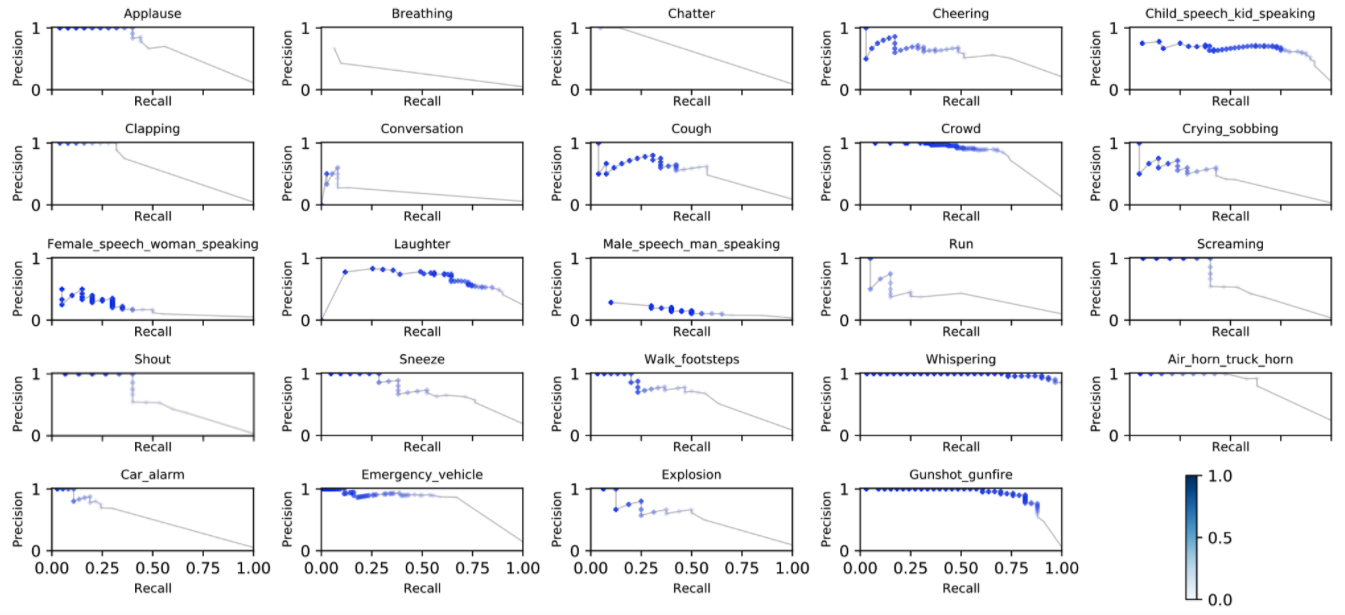
\includegraphics[width=\textwidth]{fig/precision-recall-curves.png}
    \caption{Precision-recall curves of different sound event classes at different thresholds with the CNN-Transformer-Attention system}
    \label{fig:precision-recall-curves}
\end{figure}

However, applying the optimised thresholds also consistently worsens the error rate slightly. Since the performance improvement is not consistent across all the evaluation metrics, we continue experimenting with both optimised and non-optimised thresholds in the subsequent experiments.

\subsection{Discussion for Post-Prediction Processing Methods}
From Table \ref{tab:process-res}, we can observe that averaging the frame-wise predictions in post-processing, combined with applying the optimised thresholds did improve the performance of the system. Specifically, both error rate and F1-score improved consistently across all the three model types, as compared to the previous experiment where we only applied the optimised thresholds. On the other hand, the voting scheme method generally performed worse when compared to the averaging frame-wise predictions method, which may have been attributed to its more stringent threshold scheme. Notably, applying the voting scheme method alone, as opposed to combining it with the optimised thresholds, yielded better results in comparison.\\ 

Although applying the averaging frame-wise predictions method does yield a better performing system, it should be noted that doing so increases the processing time. The total audio duration for the clips in the test set amounts to 7,470 seconds (2 hours 4 minutes 30 seconds). Taking the CNN-9-Transformer-Attention model as an example, without this additional step of averaging the frame-wise prediction, the total processing time for the test set is 25.95 seconds. When we average the frame-wise predictions, the total processing time increases to 33.68 seconds, up 29.8\% from the original. This increase in processing time may be attributed to the averaging frame-wise predictions method processing certain segments of an audio clip several times, while not doing so enables each segment of the audio clip to be processed just once. Since processing time is an important factor to consider as it affects user experience, and may be critical for certain usages, one should determine whether the averaging frame-wise prediction method is worth implementing based on their individual goals.

% From  Table  5-5  in  Section  5.2.5,  we  can  observe  that  averaging  the  frame-wise  predictions  in  post-processing,  combined  with  applying  the  optimisedthresholds did improve the performance of the system. Specifically, both errorrate and F1-score improved consistently across all the three model types,  ascompared  to  the  previous  experiment  where  we  only  applied  the  optimisedthresholds.  However, it should be noted that there is an increase in processingtime  when  the  averaging  frame-wise  predictions  method  is  used.   The  totalaudio duration for the clips in the test set amounts to 7470 seconds (2 hours4 minutes 30 seconds). Taking the CNN-9-Transformer-Attention model as anexample, without this additional step of averaging the frame-wise prediction, the total processing time for the test set is 25.95 seconds. When we average theframe-wise predictions in post-processing, the total processing time increasesto  33.68  seconds,  which  is  an  increase  of  29.8 \%  from  the  original.    Thereason for this increase in processing time is because the averaging frame-wisepredictions method processes certain segments of an audio clip several times,while not doing so enables each segment of the audio clip to be processed justonce. Since the processing time is an important factor to take into considerationas it affects the user experience, and may be critical for certain usages of thissystem,  one  should  determine  whether  the  averaging  frame-wise  predictionmethod is worth implementing based on their individual goals.

\subsection{Discussion for Performance on Lower Audio Quality Dataset}
As observed in Table \ref{tab:quality-res}, the performance of the system worsened across all the evaluation metric scores for the 8k dataset. This is as expected since the 8k dataset has a lower audio quality, compared to the 16k dataset, and has additional noise introduced for it to better mimic audio clips the system would receive as input in real-life situations. Despite the poorer results, the performance of the system trained on the 8k dataset is still comparable to that of the system trained on the 16k dataset, with only a slight increase in error rate and a slight decrease in F1-score across all three model types we tested. Specifically, the error rate increased by an average of 5.06\% and the F1-score decreased by an average of 1.87\%. As such, our system is suitable for use in real-life scenarios.

\subsection{Discussion for Performance on DCASE 2017 Dataset}
Based on Table \ref{tab:dcase2017-res}, we can observe that our trained system, namely the CNN-9-GRU-Attention model variations, managed to perform better than the state-of-the-art system \cite{kong2020sound} for the DCASE 2017 Task 4 challenge, in terms of both error rate and F1-score. However, there is a slight difference in the effect of applying frame-wise averaging, when compared to the systems trained on our project dataset. Although applying frame-wise averaging in post-prediction processing does improve the error rate consistently, it does not necessarily improve the F1-score, due to the increased false positive predictions. Since error rate is used as the main metric for evaluating and ranking systems in the DCASE 2017 Task 4 challenge, applying frame-wise averaging still works to our advantage regardless.

\subsection{Discussion for Performance on Longer Audio Clips}
As observed in Table \ref{tab:long-res}, the system which utilised the averaging frame-wise predictions post-processing method performed better than the baseline system which did not, for both of the audio clips. To better understand the reason behind this, a visual analysis for prediction results of one of the audio clips, A, alongside its groundtruth for comparison, is provided in Figure \ref{fig:audio_clip_1_result}.\\

In Figure \ref{fig:audio_clip_1_result}, at around the 20 second mark for instance, we can observe that both the baseline system and the system utilising our proposed method managed to successfully detect the presence of the 'Explosion' sound event. However, the baseline system detected a shorter duration of around 1 second, while the system utilising our proposed method detected a longer duration of around 3 second, which is more similar to that in the groundtruth, in comparison. As mentioned in Section 2.7, this discrepancy in the results is attributed to the fact that the 'Explosion' sound event is broken apart and not analysed as a whole in the baseline system, while the system utilising our proposed method is able to cover all the bases and analyse all the segment partitions with a 0.5-second stride, and finally average out the predictions to return a more optimal result.\\

\begin{figure}[!htb]
    \centering
    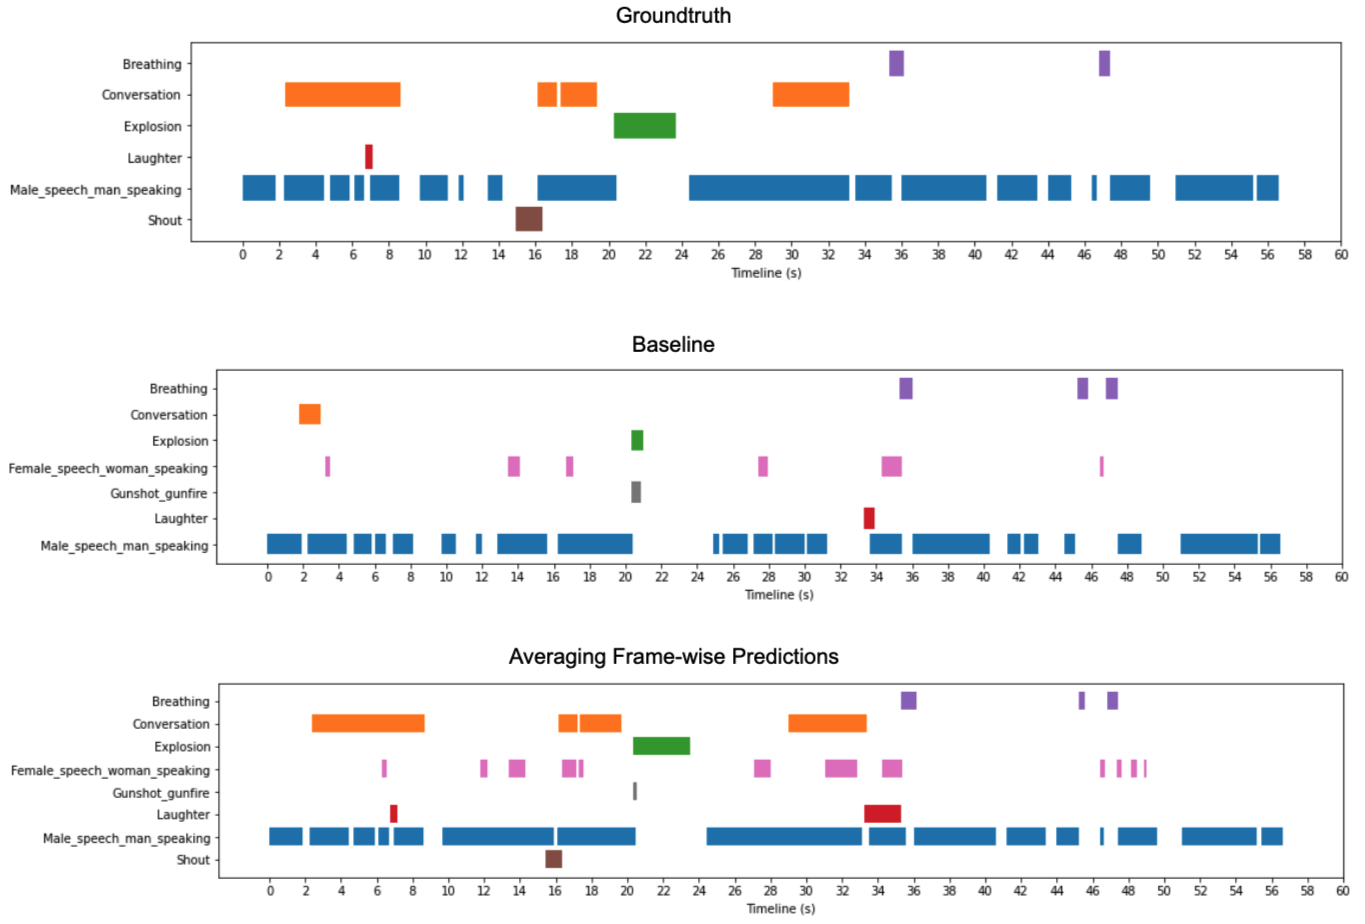
\includegraphics[width=\textwidth]{fig/audio_clip_1_result.png}
    \caption{Prediction results of audio clip A}
    \label{fig:audio_clip_1_result}
\end{figure}

\FloatBarrier %stopping float objects like images 


%=== END OF RESULTS AND DISCUSSION ===
\newpage
